\newpage
\section{Problem I: A Safe Bet}
\label{sec:Latex}
\subsection{Beschreibung der Problemdomäne}
\label{subsec:DokHeadGli}
Ein neuer durch einen Laserstrahl gesicherter Tresor wurde erfunden. Der Tresor entspricht hier einem rechteckigen Gitter. Innerhalb des Gitters befinden sich Spiegel. Es wird zwischen zwei Arten von in einem Winkel von 45 Grad diagonal orientierten Spiegeln unterschieden. Entweder sind Spiegel von der Art “\slash” oder von der Art “\textbackslash”. 

Der Laserstrahl startet immer horizontal-links in der ersten Reihe des Tresor-Gitters. Der Tresor öffnet sich, falls der Laserstrahl horizontal-rechts aus der letzten Reihe des Tresor-Gitters austritt. Die Spiegel innerhalb des Gitters können die Richtung des Laserstrahls beeinflussen.

Nachdem der Laser eingeschaltet wurde, kann der Tresor in drei mögliche Fälle eingeordnet werden.
\begin{enumerate}
  \item Sollte sich der Tresor durch den Laserstrahl öffnen lassen, ohne dass ein weiterer Spiegel hinzugefügt wurde, gilt der Tresor als \textbf{unsicher}.
  \item Ist es nicht möglich, den Tresor nur mittels des Hinzufügens eines einzelnen Spiegels zu öffnen, gilt der Tresor als \textbf{unmöglich} zu öffnen.
  \item Sollte sich der Tresor durch das Hinzufügen genau eines Spiegels öffnen lassen, so gilt dieser als \textbf{sicher}.
\end{enumerate}
Gilt ein Tresor als sicher ist zu beachten, dass es mehr als eine Möglichkeit geben kann, den Laserstrahl nur mittels eines einzigen Spiegels zum Detektor zu lenken und somit den Tresor zu öffnen. Daher wird die Anzahl aller möglichen Spiegel, welche den Tresor öffnen könnten sowie die Koordinaten des lexikographisch kleinsten Spiegels gefordert. Der lexikographisch kleinste Spiegel wird als erstes nach der Reihe und darauf nach der Spalte des Spiegels sortiert.
%
\subsection{Erkenntnisse}
\label{subsec:TextBefehle}
Trifft der Laserstrahl auf einen Spiegel, so wechselt der Laserstrahl immer seine bisherige Ausrichtung. Die Ausrichtung des Lasers ist entweder horizontal oder vertikal. Eine Richtung, aus welcher der Laserstrahl emittiert wird, kann entweder Norden, Osten, Süden oder Westen entsprechen.
\begin{figure}[h]
    \centering
    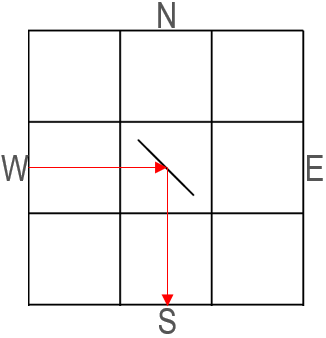
\includegraphics[width=7cm]{Bilder2/Abb3.PNG}
    \caption{Beispielhafte Spiegelung eines Laserstrahls}
    \label{fig:enter-label3}
\end{figure}

Ausgehend von dem roten Laser aus der westlichen Richtung (Abb.~\ref{fig:enter-label3}) und der Kenntnis über die Spiegelart, also “\slash” oder “\textbackslash”, kann die Ablenk-Richtung des Laserstrahls nur Süden sein. Sollte ein Laserstrahl auf einen Spiegel treffen, ist die folgende Richtung des Laserstrahls, also dessen Ablenk-Richtung, eindeutig, falls die Art des Spiegels und die Richtung, aus der der Laserstrahl emittiert worden ist, bekannt sind. 

Unterliegt der Tresor nicht dem ersten Fall, so müssen die einzelnen Spiegel bestimmt werden, welche beim Einfügen in das Tresor-Gitter den Tresor öffnen. Aus der Tresor-Beschreibung, welche Teil der erforderlichen Eingabe ist, können die Startwerte und Zielwerte des Lasers bestimmt werden. Der Start- und Endwert setzt sich aus einer \textit{x}-Koordinate und einer \textit{y}-Koordinate sowie der Richtung des Laserstrahls zusammen. Der Start des Laserstrahls ergibt sich aus den Werten (\textit{x}=1, \textit{y}=0, Osten) und der Endwert ergibt sich aus den Werten (\textit{x}=r, \textit{y}=c+1, Westen).

Anhand der Start-/Endwerte können zwei Laserstrahlen, ausgehend vom Start und ausgehend vom Ende, simuliert werden. Wenn sich die beiden Laserstrahlen schneiden, muss dies ein horizontaler Abschnitt vom Start mit einem vertikalen vom Ende oder ein vertikaler Abschnitt vom Start mit einem horizontalen vom Ende sein. Beide Laserstrahlen erreichen den Schnittpunkt, jedoch müssen ihre Ausrichtungen unterschiedlich sein. Folglich reicht ein einzelner Spiegel, damit der Laserstrahl vom Start bis zum Ende reicht. Aufgrund der Eigenschaft, dass die Spiegel die Laserstrahlausrichtung verändern, reicht genau ein Spiegel aus. 

Jeder Schnittpunkt der beiden Laserstrahlen repräsentiert einen möglichen Spiegel, welcher den Tresor öffnen würde. Sollte kein Schnittpunkt existieren, so wäre es nicht möglich, mit nur einem Spiegel den Tresor zu öffnen und der Tresor unterliegt dem zweiten Fall.
%
\subsection{Modellierung des Problems}
\label{subsec:TextBefehle}
Die in der Tresor-Beschreibung gegebenen Spiegel können innerhalb zweier Mengen gespeichert werden. Eine Menge repräsentiert alle Zeilen und speichert für jede Zeile das Vorkommen aller Spiegel innerhalb dieser. Es werden die Art des Spiegels und die zugehörige Spalte des Spiegels gespeichert. Die zweite Menge, welche alle Spalten repräsentiert, kann analog erstellt werden. Ein Laserstrahl kann durch gegebene Spiegel bezüglich seiner Richtung beeinflusst werden und besteht daher potenziell aus mehrere horizontalen und vertikalen Linien. Eine Feld-Datenstruktur speichert, wie viele horizontale Linien sich innerhalb eines Bereiches befinden.
%
\subsection{Lösungsansatz}
\label{subsec:Abb}
Eine Eingabedatei kann mehrere Tresor-Beschreibungen beinhalten. Anfangs beschreibt ein Quadrupel (\textit{r}, \textit{c}, \textit{m},\textit{n}) die Anzahl der Reihen (\textit{r}) und Spalten (\textit{c}) des Tresor-Gitters. Die nachfolgenden \textit{m}- und \textit{n}-Zeilen beschreiben die Koordinaten der "\slash”-Spiegel beziehungsweise der “\textbackslash”-Spiegel.

Anfangs werden die zwei Mengen “rows” und “columns” erstellt. Eine Menge verweist mittels Schlüssel auf Paare. In der Menge “rows” gibt es für jede Zeile einen eindeutigen Schlüssel. Der \textit{i}-te Schlüssel aus der Menge “rows” entspricht der \textit{i}-ten Zeile innerhalb des Tresor-Gitters. Die \textit{i}-te Zeile entspricht der \textit{x}-Koordinate des Spiegels. Jedes Paar der Menge “rows”, besteht aus der \textit{y}-Koordinate und der Art des jeweiligen Spiegels innerhalb der Zeile. Die \textit{y}-Koordinate entspricht der Spalte des Spiegels. Analog wird die Menge “columns” erstellt. 

Geraden innerhalb des Tresor-Gitters werden als Linien bezeichnet. Ein Laserstrahl wird durch mehrere Linien dargestellt. Eine Linie beinhaltet die Informationen “xlow”, “xhigh”, “ylow” und “yhigh”. Da Linien eindimensional sind, entspricht bei horizontalen Linien “xlow” gleich “xhigh” und bei vertikalen “ylow" gleich “yhigh”.
\begin{figure}[h]
    \centering
    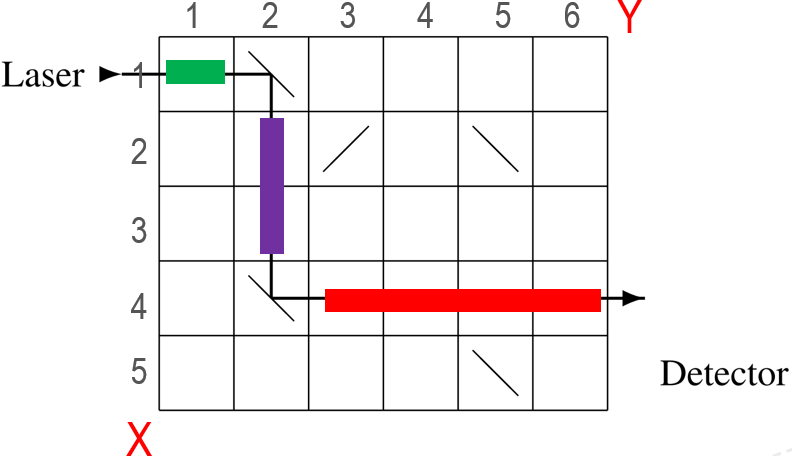
\includegraphics[width=10cm]{Bilder2/Abb4.PNG}
    \caption{Beispielhafte Linien eines Laserstrahls}
    \label{fig:enter-label4}
\end{figure}

Anhand der Abbildung~\ref{fig:enter-label4} ist zu erkennen, wie die Werte einer konkreten Linie bestimmt werden. Für die horizontale, rote Linie (Abb.~\ref{fig:enter-label4}) wären die Werte xlow=4, ylow=3, xhigh=4 und yhigh=6. Um die einzelnen Linien zu bestimmen, werden die aktuellen Koordinaten des Lasers benötigt und die aktuelle Richtung eines von dem Laser emittierten Laserstrahls. Beim Start ist der Laserstrahl aus Westen kommend ausgerichtet und die Koordinaten des Lasers sind (\textit{x}=1, \textit{y}=0). Anhand dieser Informationen kann für horizontale Linien innerhalb der “rows”-Menge nachgeschaut werden, bei welchen Koordinaten der Laserstrahl auf einen Spiegel trifft. Da die \textit{x}-Koordinate die aktuelle Zeile und somit den Schlüssel der Menge angibt, muss nur überprüft werden, wann der nächste Spiegel bezüglich der aktuellen \textit{y}-Koordinate (der Spalte) kommt. 
Für vertikale Linien wird die “columns”-Menge geprüft, ob innerhalb der aktuellen Spalte (\textit{y}-Koordinate) ein weiterer Spiegel folgt, ausgehend von der aktuellen Zeile (\textit{x}-Koordinate). Bezüglich der Richtung des Laserstrahls, kann entweder links oder rechts von der aktuellen Spalte beziehungsweise unterhalb oder oberhalb der aktuellen Zeile gesucht werden. Alle Linien werden dabei innerhalb zwei dynamischer Felder, getrennt bezüglich horizontaler und vertikaler Linien, gespeichert. Sollte es keinen Spiegel innerhalb der Zeile/Spalte mehr geben, dann ist dies die letzte Linie und der Laserstrahl endet.

Sobald der Laserstrahl, ausgehend vom Start emittiert wurde, muss überprüft werden, ob dieser bereits den Tresor öffnet. Um den Tresor zu öffnen, muss der Laserstrahl mit den Koordinaten des Detektors enden. Sollte die Koordinaten des Laserstrahls \textit{r} und \textit{c+1} entsprechen, ist der Laserstrahl am Detektor angekommen. Der Tresor wäre unsicher. Die Ausgabe für den Tresor kann direkt nach dieser Feststellung getätigt werden.

Handelt es sich jedoch um keinen unsicheren Tresor, muss ausgehend vom Ende ein weiterer Laserstrahl simuliert werden. Die Erstellung der horizontalen und vertikalen Linien ist analog, allerdings gilt es zu beachten, dass die Linien vom Start und Ende in getrennten dynamischen Feldern gespeichert werden. Daraus resultieren zwei Felder für horizontale Linien und zwei Felder für vertikale Linien.

Zum Auffinden der Schnittpunkte wird der Plane-Sweep-Algorithmus benutzt. Dieser verwendet Events, um mögliche Schnittpunkte ausfindig zu machen. Ein Event beinhaltet die Information, ob dieses zu einer vertikalen Linie gehört, einen “value”, zwei Werte ("low", "high") zur \textit{x}-Achsen Intervalleingrenzung und einen “add”-Wert. Der “value” entspricht der y-Koordinate der Linie. Anhand der \textit{y}-Koordinate werden alle Events aufsteigend sortiert. 

Zu Beginn werden alle Events erstellt. Jede horizontale Linie benötigt zwei Events. Der erste Punkt repräsentiert den Start der horizontalen Linie auf der \textit{y}-Achse. Mittels des zweiten Events wird das Ende dieser horizontalen Linie gekennzeichnet. Vertikale Linien erhalten nur ein Event, da diese nur eine \textit{y}-Koordinate beinhalten. Die Events werden aufsteigend nach ihrem “value” sortiert. Die Sortierung repräsentiert die Auslöse-Reihenfolge der Events. Falls es sich um ein horizontales Event handelt, wird immer das Feld, welches die horizontalen Linien speichert, verändert. Die Veränderung ist abhängig davon, ob es sich um den Start oder das Ende der horizontalen Linie handelt. Beim Aufruf eines vertikalen Events wird über die \textit{x}-Achse das Intervall der vertikalen Linie gebildet. Sollte im Feld, innerhalb des Intervalls, ein horizontales Event gestartet und noch nicht beendet sein, ist dies anhand der Feldeinträge erkennbar. Somit muss die vertikale Linie von einer horizontalen Linie geschnitten werden.

Die Datenstruktur des Binary Indexed Tree ermöglicht eine passende Verwaltung des Feldes. Demnach ist jeder Index des Feldes für einen Bereich von Indizes zuständig. Ein Index muss für seinen Bereich die Summe aller Einträge speichern. Der Bereich kann durch die binäre Darstellung des Index  ermittelt werden. Verändert sich ein Index, indem ein horizontales Event aufgerufen wird, können alle Indizes, welche ebenfalls ihren Summe anpassen müssen, über die Addition des “least significant bit” ermittelt werden. Für die Ermittlung einer Präfixsumme können zusätzlich zum ursprünglichen Index-Wert alle Werte der Indizes addiert werden, welche nach Subtraktion des “least significant bit” folgen. Eine Summe über ein Intervall \textit{xl} bis \textit{xr} lässt sich mittels der Subtraktion der Präfixsumme von \textit{xr} minus der Präfixsumme von \textit{xl}-1 berechnen.

Ein Index repräsentiert eine \textit{x}-Koordinate. Horizontale Linien haben nur einen \textit{x}-Wert. Der entsprechende “add” Wert des horizontalen Events wird auf den passenden Index addiert. Beim ersten horizontalen Event wird der Index (\textit{x}-Koordinate) um eins erhöht. Folglich erhöht sich die Präfixsumme innerhalb des Feldes, ab diesem Index. Die horizontale Linie hat begonnen. Beim zweiten Event wird der Index um eins erniedrigt. Ab diesem Event ist die horizontale Linie beendet. Diese wird nicht mehr in der Präfixsumme berücksichtigt und kann daher ab diesem Zeitpunkt in keinem Intervall gefunden werden. Es wird ausgeschlossen, dass nachfolgende vertikale Linien eine schon beendete horizontale Linie schneiden. Vertikale Events umfassen ein \textit{x}-Achsen-Intervall. Das Feld berechnet für das gegebene Intervall eine Summe. Sollte diese Summe größer null sein, läuft mindestens eine horizontale Linie durch das Intervall der vertikalen Linie. Diese beiden Linien bilden folglich einen Schnittpunkt. 

Nachdem die horizontalen Linien vom Start mit den vertikalen Linien vom Ende und die vertikalen Linien vom Start mit den horizontalen Linien vom Ende auf Schnittpunkte geprüft wurden, erfolgt die Ausgabe. Gibt es keinen Schnittpunkt, ist der Tresor unmöglich zu öffnen. Sollte es Schnittpunkte geben, so wird die Anzahl der Schnittpunkte aufaddiert. Direkt nachdem ein Schnittpunkte gefunden wird, welcher lexikographisch kleinere Koordinaten als der aktuell kleinste Schnittpunkt besitzt, wird dieser Schnittpunkt zum lexikographisch kleinsten. Der lexikographisch kleinste Spiegel entspricht dem lexikographisch kleinsten Schnittpunkt. Für einen sicheren Tresor kann somit die Summe aller möglichen einzelnen Spiegel und die Koordinaten des lexikographisch kleinsten Spiegels ausgegeben werden.
%
\subsection{Implementierung}
\label{subsec:TextBefehle}
Die Implementierung beinhaltet eine vereinfachte Darstellung der benötigten Klassen und Methoden. Eine vollständige Implementierung in C++ ist im Anhang zu finden.
\begin{lstlisting}
tree = Feld zum Speichern der horizontalen Events 
lowestX = x-Koordinate des lexikographisch kleinsten Schnittpunkts 
lowestY = y-Koordinate des lexikographisch kleinsten Schnittpunkts

rows = Menge der Zeilenspiegel
columns = Menge der Spaltenspiegel 

//horizontale/vertikale Linien
class line{
    public:
        //Parameter einer Linie
        int xlow, ylow, xhigh, yhigh;
}

//Events 
class event{
    public:
        //Parameter eines Events
        bool vertical;
        int value, low, high, add;

        bool operator < (const event &other)const{
            //Anordnungsrelation der Events 
        }
};

//Emittiert einen Laserstrahl
void laserbeam(hori, verti, x, y, dir){ 
    while(Laserstrahl trifft nicht den Gitterrand){
        //überprüfe die aktuelle Richtung
        if(dir == W){
            auto it = nächster Spiegel innerhalb des passenden Sets

            if(it == rows[x].begin()){
                //Laserstrahl trifft den Gitterrand
            }else{
                //Bestimmung neuer Richtung
            }
        }else if(dir == S){
            analog
        }           
        }else if(dir == E){
            analog
        }
        }else if(dir == N){
            analog
        }
        //Speichern der Linien getrennt nach horizontalen/vertikalen
        if(nextX == x){
            hori.emplace_back(line{x, min(y, nextY)+1, x, max(y, nextY)-1});
        }else if(nextY == y){
            verti.emplace_back(line{min(x, nextX)+1, y, max(x, nextX)-1, y});
        }
        //nächsten Koordinaten
        x = nextX;
        y = nextY;
    }
    //prüft, ob der Laserstrahl im Detektor endet
    if(x == r && y == c+1){
        without = true;
    }
}

void update(int pos, int value){
    addiert einen übergebenen Wert auf alle Positionen eines Binary Indexed Tree
}

big prefixSum(int pos){
    berechnet eine Präfixsumme bis zu einer gegebenen Position
}

big intervalSum(int left, int right){
    //berechnet Intervallsummen vertikaler Events
    return prefixSum(right) - prefixSum(left-1);
}

//berechnet Schnittpunkte 
big intersections(hori, verti){
    e = Liste aller Events
    //erstellt alle horizontalen und vertikalen Events
    for(auto h : hori){
        e.emplace_back(false, h.ylow, h.xlow, h.xlow, 1);
        e.emplace_back(false, h.yhigh, h.xlow, h.xlow, -1);
    }
    for(auto v : verti){
        e.emplace_back(true, v.ylow, v.xlow, v.xhigh, -1);
    }
    sort(e.begin(), e.end());
    //iteriert über alle sortierten Events
    for(auto e1 : e){
        //vertikales Event
        if(e1.vertical){
            int low = e1.low;
            int high = e1.high;
            inter = Intervallsumme der x-Koordinaten des vertikalen Events
            //entspricht die Intervallsumme mind. 1 => Schnittpunkt
            if(inter <= 0){
                continue;
            }
            while(low < high){
                int mid = (low + high)/2;
                //Binäre Suche der exakten Koordinaten des Schnittpunkts
            }
            //Vergleich des Schnittpunkts mit dem aktuell lexikographisch 
            //kleinsten Schnittpunkts
                     
            result = Speichert die Anzahl der gefundenen Schnittpunkte

        //horizontales Event
        }else{
            //Feldveränderung
        }
    }
    return result;
}   
\end{lstlisting}
%
\subsection{Laufzeit}
\label{subsec:TextBefehle}
Die Sets “rows” und “columns” speichern Spiegelinformationen. Dazu wird pro Set jeder Spiegel einmalig benötigt. Es gibt (\textit{m}+\textit{n})-viele Spiegel, folglich unterliegt die Initialisierung der Sets einer konstanten Laufzeit von $\mathcal{O}(m+n)$, da \textit{m} und \textit{n} bekannte Konstanten sind. Innerhalb des Tresor-Gitters kann es bis zu \textit{rc} Linien geben, welche einem Laserstrahl zugeordnet werden. Somit kann es bis zu $\mathcal{O}(rc)$ Zeit benötigen, um einen Laserstrahl zu emittieren. Ausgehend von \textit{e}-vielen Events für eine Tresor-Beschreibung, benötigt der Plane-Sweep-Algorithmus für das Ausführen der "\text{update}"\text{-Funktion} $\mathcal{O}(elog(e))$ und für die Berechnung einer Intervallsumme ebenfalls $\mathcal{O}(elog(e))$ [2]. Folglich werden alle Schnittpunkte innerhalb einer Laufzeit von $\mathcal{O}(elog(e))$ berechnet. Zusammengefasst ergibt sich eine asymptotische Laufzeit pro Tresor-Beschreibung von $\mathcal{O}(rc+elog(e))$. 
\subsection{Testergebnisse}
\label{subsec:TextBefehle}
Die Implementierung wurde erfolgreich mittels des Online-Judge-Tools getestet. Darüber hinaus wurden alle bereitgestellten Testfälle mithilfe eines Python-Skripts ausgeführt. Die Laufzeit pro Testfall in Sekunden ist in einer Tabelle im Anhang aufgeführt. Zur Bestätigung ist ein Screenshot der Ergebnisse aus dem Online-Judge beigefügt.
%